\lecture{Synchronisation and Deadlock}{13:00}{17/10/23}{Tamer Elboghdadly}

\section*{Synchronisation}

\begin{itemize}
  \item Mutual Exclusion is just one type of synchronisation, but there are others, such as:
  \begin{itemize}
    \item Messaging - Threads can send messages to each other. The recieving thread cannot continue until it gets a message from the sending thread
    \item Join synchronisation - The parent thread can wait for the child thread to terminate
    \item Barrier synchronisation - All threads must wait for all other threads to reach a barrier operation before they can continue
  \end{itemize}
  \item Semaphores can be used to achieve multiple types of synchronisation
  \begin{itemize}
    \item When using for Mutual Exclusion, the semaphore usually starts at 1
    \item It could start at 0, and when a thread completes an operation, it raises the semaphore using V, allowing another thread to know it has completed an operation
    \item This would allow you to guarantee the order in which the operations are run, rather than just that they don't run at the same time
  \end{itemize}
\end{itemize}

\section*{Deadlock}

\begin{itemize}
  \item The resources of a computer can only be accessed by one thread at a time
  \item Mutual Exclusion is one example of this, as only one thread can access the areas in memory belonging to a data structre at a time
  \item Other examples are devices such as a printer or scanner
  \item A situation which could cause a deadlock is as follows
  \begin{itemize}
    \item Two threads, A and B, need access to resources R and S
    \item They both need access to the resources, but attempt to acquire them in different orders
    \item Thread A acquires R and B acquires S
    \item Thread A now attempts to acquire S, and B attempts to acquire R
    \item Each thread is waiting for the other thread to release the resource
    \item This causes a complete deadlock as neither thread will finish and release the resource
  \end{itemize}
\end{itemize}

\subsection*{Deadlock Modelling}

\begin{itemize}
  \item Resource deadlock can be modelled using a resource allocation graph
  \item This shows
  \begin{itemize}
    \item Which processes are requesting which resources
    \item Which resources have been assigned to which processes
  \end{itemize}
  \item If this graph contains a cycle, there will be a deadlock. If not, there won't be a deadlock
\end{itemize}

\begin{figure}[h]
  \centering
  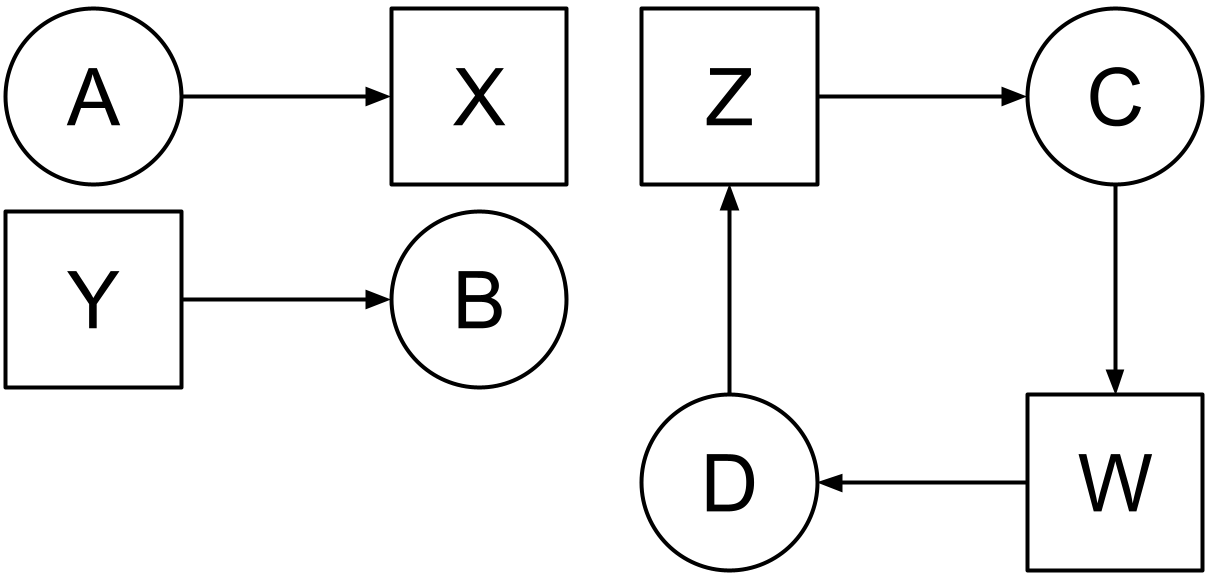
\includegraphics[width=0.8\textwidth]{resource-allocation-graph.png}
  \caption{A resource allocation graph - Process A is waiting for resource X; Resource Y is assigned to process B; Process C and D are in a deadlock, waiting for resources Z and W}
\end{figure}

\subsection*{Deadlock Detection and Recovery}

\begin{itemize}
  \item This is a process which allows the system to enter a deadlocked state
  \item A deadlock detection algorithm is run periodically
  \item If a deadlock is detected by finding a cycle in the resource allocation graph, process that make up the cycle are randomly killed until the deadlock is resolved
  \item Any remaining processes are allowed to use the requested resources
  \item This is very inefficient and may result in data loss depending upon the type of processes being killed
  \item It is commonly used in relational databases, as any transactions which create a deadlock can be rolled back, allowing the system to continue
\end{itemize}

\subsection*{Deadlock Avoidance}

\begin{itemize}
  \item It would be better if the system never entered a deadlock state
  \item This works as follows:
  \begin{itemize}
    \item The system analyses the resource usage of all threads of the system
    \item This allows it to predict when threads will need access to a specific resource
    \item If two threads need access to two resources in confliting orders, the system will pause one thread until the other is finished with both resources
    \item This avoids entering an unsafe execution path in which a deadlock is guaranteed
  \end{itemize}
  \item One such deadlock avoidance algorithm is Dijkstra's Banker's algorithm
  \begin{itemize}
    \item All processes declare which resources they may need access to, and how much of said resources they may need
    \item The algorithm then keeps track of the current allocation for each process
    \item When a request for more resources is received, it pretends to honor the request, before attempting to fulfill the needs of all other processes
    \item If it is unsafe to do so, deny the request, else grant it
  \end{itemize}
\end{itemize}